\chapter{Catalan Objects}
The Catalan numbers are possibly the most ubiquitous sequence of numbers in mathematics.  
Named for mathematician Eugene Charles Catalan, the $n\thh$ Catalan number can be succinctly defined as the number of ways of triangulating a convex polygon with $n+2$ sides.  The Catalan numbers can also be defined mathematically as follows:

\begin{align}
    \mathcal{C}_n &= \frac{(2n)!}{n!(n+1)!} =1, 1, 2, 5, 14, 42, 132, \ldots & \text{OEIS} A000108
\end{align}

The Catalan numbers count a remarkable number of interesting and useful combinatorial objects in bijective correspondence with triangulation of $n$-gons. Combinatorial objects counted by the Catalan numbers are referred to as \emph{Catalan objects}.   Richard Stanley's book \emph{Catalan Numbers} gives hundreds of examples of Catalan objects  as well as including a thorough history on the numbers and their study \cite{stanley2015catalan}. This thesis will focus on three Catalan objects: Dyck words, binary trees, and ordered trees. 

\begin{figure}[H]
\begin{center}
\begin{tikzpicture}
    \coordinate (a) at (-0,1);
    \coordinate (b) at (0.951,0.309);
    \coordinate (c) at (0.587,-0.809);
    \coordinate (d) at (-0.587,-0.809);
    \coordinate (e) at (-0.951,0.309);


\matrix[column sep=0.8cm,row sep=0.5cm]
{
    \pslice{a/d,a/c} &
    \pslice{b/e,b/d} &
    \pslice{c/a,c/e} &
    \pslice{d/b,d/a} &
    \pslice{e/c,e/b} \\
};
\end{tikzpicture}
\end{center}
    \caption{The $\mathcal{C}_3$=5 triangulations of a polygon with $3+2=5$ sides.}
\label{fig:}
\end{figure}

\section{Dyck Words and Paths}
The language of binary Dyck words is the set of binary strings that satisfy the following conditions: The string has an equal number of ones and zeroes and each prefix of the string has at least as many ones as zeroes.  The number of distinct Dyck words with $n$ ones and $n$ zeroes is equal to $\mathcal{C}_n$.

Two common interpretations of Dyck words are in terms of balanced parentheses and in terms of paths in the Cartesian plane. If each one in a Dyck word is taken to represent an open parenthesis and each 0 a closing parenthesis, the Dyck language becomes the language of balanced parentheses.  Alternatively, the Dyck language can be interpreted as the set of paths in the Cartesian plane using $(1,1)$ (northeast) and $(1,-1)$ (southeast) steps that start at $(0,0)$ and never go below the x axis. In this case, each 1 in a Dyck word represents a $(1,1)$ step and each 0 represents a $(1,-1)$ step.

Figure $\ref{fig:Dycks}$ gives an illustration of each of these interpretations of Dyck words for $n=4$.

\begin{figure}
    \centering
    \begin{tabularx}{0.55\textwidth}{>{\hsize=0.4\hsize}C >{\hsize=0.2\hsize}C >{\hsize=0.2\hsize}C   }
       \thead{Dyck Path} & \thead{Dyck Word} & \thead{Parentheses} \\ \hline 

\LukaTable[4]{2,2,2,2,0,0,0,0} & 11110000 & (((())))\\
\LukaTable[3]{2,0,2,2,2,0,0,0} & 10111000 & ()((()))\\
\LukaTable[3]{2,2,0,2,2,0,0,0} & 11011000 & (()(()))\\
\LukaTable[3]{2,2,2,0,2,0,0,0} & 11101000 & ((()()))\\
\LukaTable[2]{2,0,2,2,0,2,0,0} & 10110100 & ()(()())\\
\LukaTable[2]{2,2,0,2,0,2,0,0} & 11010100 & (()()())\\
\LukaTable[2]{2,0,2,0,2,2,0,0} & 10101100 & ()()(())\\
\LukaTable[2]{2,2,0,0,2,2,0,0} & 11001100 & (())(())\\
\LukaTable[3]{2,2,2,0,0,2,0,0} & 11100100 & ((())())\\
\LukaTable[2]{2,0,2,2,0,0,2,0} & 10110010 & ()(())()\\
\LukaTable[2]{2,2,0,2,0,0,2,0} & 11010010 & (()())()\\
\LukaTable[1]{2,0,2,0,2,0,2,0} & 10101010 & ()()()()\\
\LukaTable[2]{2,2,0,0,2,0,2,0} & 11001010 & (())()()\\
\LukaTable[3]{2,2,2,0,0,0,2,0} & 11100010 & ((()))()\\

    \end{tabularx}
    \caption{The $\mathcal{C}_4=14$ Dyck words of order 4}
    \label{fig:Dycks}
\end{figure}
%TODO: PATHS
% In addition to balanced parentheses, Dyck words of length $2n$ are also in bijective correspondence with extended binary trees with $n$ internal nodes. 
% Given an extended binary tree $B$ with n internal nodes, a Dyck word can be obtained by traversing B in preorder and recording each internal node as a $1$ and each leaf with a $0$, ignoring the final leaf of the tree.

% \begin{figure}
%     \centering
%     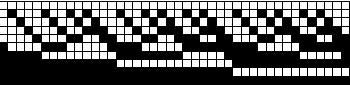
\includegraphics[width=.8\textwidth]{CD5.pdf}
%     \caption{The $\mathcal{C}_5=42$ Dyck words of order 5}
%     \label{fig:dyck5}
% \end{figure}

% TODO

% \section{Grid Paths}
\section{Binary Trees}

The language
\section{Ordered Trees}
\section{Bijections}
This algorithm will use the bijection between ordered trees and Dyck words specified in \cite{stanley2015catalan}. The bijection described by Stanely is as follows:
\footnote{ Stanley's text refers to ordered trees as \emph{plane trees} and Dyck words as \emph{ballot sequences}} 


Given an ordered tree T with $n+1$ nodes: Traverse T in preorder.  Whenever going ``down" an edge, or away from the root, record a 1.  Whenever going ``up" an edge, or towards the root, record a 0.  The resulting binary sequence is a Dyck word D corresponding to the ordered tree T. 

This process can be inverted as follows: 

As before, let $D=d_1...d_{2n}$ be a dyck word of order n with $n > 0$. Construct an ordered tree T via the following steps. 

Create a root node of T.  Keep track of a current node $curr$; set $curr=root$.

\begin{itemize}
    \item For each $d_i$ such that $1 \le i \le 2n$ %TODO: QUESTION: is it clear that this goes 1,2,3,...,2n?
	\begin{itemize}
	    \item if $d_i=1$: append a rightmost child $ch$ to $curr$'s children; set $curr=ch$
	    \item if $d_i=0$, set $curr$ equal to $curr$'s parent.
	\end{itemize}
	%TODO: QUESTION: do I need to prove this? It seems like Stanely assumed this was basically obvious 

\end{itemize}
Figure \ref{ordered_tree_bijection_illustration} demonstrates both directions of this process. Note that each $t_i$ with $1 \le i \le n$ in a preorder traversal of T corresponds to the $i^{\underline{th}}$ 1 in D.

\begin{figure}
    \centering
    % TODO: degree three, color binary bits to illustrate correspondence
    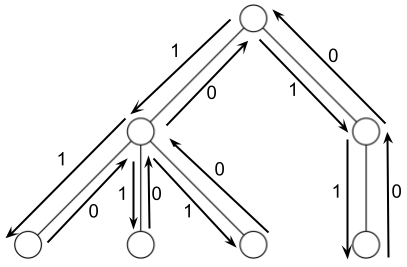
\includegraphics[width=0.5\textwidth]{otreebij.png}
    \caption{An ordered tree with $6+1=7$ nodes corresponding to the order 6 Dyck word $110101001100$.}
    \label{ordered_tree_bijection_illustration}
\end{figure}

%TODO: Combine the above and below figures?? Have them adjacent to each other?

In addition to the above bijection, we define the following functions relating to ordered trees, Dyck words, and the correspondence between them.

\begin{itemize}
    \item Let $\otree{D}$ and $\dyck{T}$ be functions that convert a Dyck word to an ordered tree and an ordered tree to a Dyck word respectively via the above process.
    \item Let $\depth{t_i}=$ length of path between root and $t_i$. $\depth{root}=0$
    \item Let $\oneindex{D}{i}=$ be the index of the $i\thh{}$ one in D.
\end{itemize}

\bigskip

\begin{figure}
    \centering
    $T=$

    \begin{tikzpicture}[every tree node/.style={draw,circle},sibling distance=10pt, level distance=40pt]
	\tikzset{edge from parent/.style={draw, edge from parent path=
	{(\tikzparentnode) -- (\tikzchildnode)}}}
	\Tree [.\node[style={fill=lightpurple}]{}; [.\node[style={fill=lightpurple}]{G}; [.\node[style={fill=lightpurple}]{P};[.\node[style={fill=lightpurple}]{L}; [.\node[style={fill=lightpurple}]{}; [.\node[style={fill=lightpurple}]{}; [.\node[style={fill=lightpurple}]{F}; ] ] ] ] [.\node{O}; [.\node{}; ] ] [.\node{}; ] ] [.\node{}; [.\node{}; ] ] ] ]
    \end{tikzpicture}

    $D=[1, 1, 1, 1, 1, 1, 0, 0, 0, 0, 1, 1, 0, 0, 1, 0, 0, 1, 1, 0, 0, 0]$
    \caption{An ordered tree with 12 nodes corresponding to the Dyck word 1111110000110010011000.  The left down path of T is highlighted in purple. }
    \label{exampleotree}
\end{figure}

The following remarks can be derived from the bijection between ordered trees and Dyck words.


\begin{remark}
    $t_i$ corresponds to the $i$th one in D for $1 \le i \le n$
\end{remark}
\begin{proof}
    Recall the method of constructing an ordered tree from a Dyck word.  Each one in D creates a new node; zeroes in D do not create nodes.  Generating an ordered tree from a Dyck word generates the nodes of the tree in preorder.  Thus, $t_i$ corresponds to the $i$th one in D for $1 \le i \le n$.
\end{proof}

\begin{remark} The difference in depths between nodes $t_i$ and $t_{i-1}$ is equal to one minus the number of zeroes between the $(i-1)^{\underline{st}}$ and $i\thh$ and  ones in $D$


    % TODO: eqref?
\end{remark}
\begin{proof}

    This remark can be stated formally as 

    \begin{equation} \label{eq:depthformula} 
    	\depth{t_i} - \depth{t_{i-1}}=1-(\oneindex{D}{i}-\oneindex{D}{i-1} - 1) 
    \end{equation}
    

    % or equivalently, 

    % \begin{equation} \label{eq:indexformula} 
    % 	\oneindex{D}{i} = \oneindex{D}{i-1} + \depth{t_{i-1}} - \depth{t_i} + 2
    % \end{equation}
    

    Note that $(\oneindex{D}{i}-\oneindex{D}{i-1}-1)$ is equal to the number of zeroes between the $i\thh$ and $(i-1)^{\underline{st}}$ ones in D.  % Therefore, this rule can be informally described as follows:

    % The depth of $t_i$ is the depth of $t_{i-1}$ plus 1 minus the number of zeroes between the $(i-1)\thh$ and $i\thh$ ones in D

    % The number of zeroes between the $i\thh$ and $(i-1)\thh$ ones in $D$ is equal to one plus the depth  $\depth{t_i}$ minus $\depth{t_{i-1}}$

    This follows naturally from the bijection between Dyck words and ordered trees.  Each zero corresponds to a step up in the tree before adding the next child.  

    If there are zero zeroes between the $i\thh$  and $(i-1)^{\underline{st}}$ ones in D, $t_i$ is a child of $t_{i-1}$; $\depth{t_i}=\depth{t_{i-1}}+1$

    If there is one zero between the $i\thh$  and $(i-1)^{\underline{st}}$ ones in D, $t_i$ is a child of $t_{i-1}$'s parent; $\depth{t_i}=\depth{t_{i-1}}+1$.  

    Each subsequent zero between $t_{i-1}$ and $t_i$ decreases $\depth{t_{i}}$ by one.  Thus, the depth of $t_i$ is the depth of $t_{i-1}$ plus 1 minus the number of zeroes between $t_{i-1}$ and $t_{i}$.
\end{proof}
% \bigskip


\begin{remark}A preorder listing of $\depth{t_i} $ for each $ t_i \in T$ can be used to construct a Dyck word. \label{re:construct_dyck}

\end{remark} 
\begin{proof}
    % This follows from Remark \ref{re:depthformula}, as it implies that for any $i,i+1 \le n$, $\oneindex{D}-\oneindex{$ 

    Let $T=t_0,t_1,...t_n$ be a preorder traversal of T.  Note that $t_0$ is the root of $T$

    Construct D as follows: 

    \begin{itemize}
	% \item skip $t_0$
	\item Let $D=\epsilon$ % clear that this is empty string?
	\item For each $t_i$, $1\le i \le n$
	    \begin{itemize}
		\item Append a 1 to $D$
		\item Append $1-\depth{t_{i}}+\depth{t_{i-1}}$ zeroes to D.
	    \end{itemize}
	\item Append $\depth{t_{n}}$ zeroes to D. 
    \end{itemize}
\end{proof} 

% TODO: move to ch 3, or its own chapter?
\section{Cool Lex Order on Dyck Paths and Binary Trees}
Ruskey and Williams found the following successor rule for enumerating binary Dyck words, dubbed ``CoolCat" due to its use of a cool-lex order to generate (cat)alan objects \cite{ruskey2008generating}:
We will use $\mathbf{B}_n$ to denote binary Dyck words with $n$ ones and $n$ zeroes.  Note that the length of any string in $\mathbf{B}_n$ is thus $2n$.

\noindent Let $D \in \mathbf{B}_n$

\noindent Let the $i$th prefix shift of D, denoted by $\preshift{D}{i}$, be a function that rotates the second through ith symbols of D one to the right circularly.  More formally, 

\noindent $\preshift{d}{i}=d_1,d_i,d_2,...,d_{i-1},d_{i+1},d_{i+2},...,d_{2n}$


\noindent Let $k$ be the index of the 1 in the leftmost $01$ substring in $D$ if it exists. Note that if $D$ has no $01$ substring, then $D=1^n0^n$.  The successor rule for $D$ is as follows:


\begin{subnumcases}{\coolCat{D} = \label{eq:prefixDyck_simple}}
	\preshift{D}{2n} & \text{if $D$ has no $01$ substring}\\
	\preshift{D}{k+1} & if $\preshift{D}{k+1} \in \mathbf{B}_n$\\
	\preshift{D}{k} & otherwise
\end{subnumcases}

Ruskey and Williams's algorithm can also enumerate a broader set of strings: The algorithm enumerates any set $\mathbf{B}_{s,t}$ where any $D \in \mathbf{B}_{s,t}$ has s zeroes and t ones and satisfies the constraint that each prefix of D has as many ones as zeroes.  This is slightly broader than the language of Dyck words, as it does not have the requirement that a string have an equal number of ones and zeroes.
We will focus on $\mathbf{B}_n$  languages due to their correspondce with Dyck words and therefore other catalan objects.

Evaluating whether $\preshift{D}{k+1} \in \mathbf{B}_n$ can be determined by looking $D_{k+1}$ and the sum of the first k symbols of D:  

Let $D'=$ $\preshift{D}{k+1}$

Note that we know $D \in \mathbf{B}_n$.  

Since preshift only rotates symbols, $D'$ will automaticallly satisfy the requirement that strings in $\mathbf{B}_n$ must have an equal number of zeroes and ones since D satisfied that requirement. Thus, $D' \in \mathbf{B}_n$ will be determined by whether or not all prefixes of $D'$ have at least as many ones as zeroes.  

If $D_{k+1}$ is a 1, then  for all i, the $i\thh$ prefix of $D'$ will have at least as many ones as the $i\thh$ prefix of D.  Thus, $D'$ must be $\in \mathbf{B}_n$, as rotating a 1 to earlier in the string will never invalidate the requirement that every prefix of the string has at least as many ones as zeroes.  

Note that the $k\thh$ prefix of D must be of the form $1^a0^b1$, as otherwise there would be an earlier $01$ prefix.  Fruthermore, $a\ge b$ as otherwise the bth prefix of D would have more zeroes than ones and D would not be a valid Dyck word.

If $D_{k+1}$ is a 0, then $D' \notin \mathbf{B}_n$ if and only if rotating a 0 to index 2 creates a prefix of D with more zeroes than ones.  This will only happen if the $(k-1)\thh$ prefix of D is exactly $1^{\frac{k-1}{2}}0^{\frac{k-1}{2}}$.  

Therefore, $\preshift{D}{k+1} \in \mathbf{B}_n \iff D_{k+1}=1$ or $D$ starts with more than $\lfloor \frac{k-1}{2} \rfloor$ ones 

\begin{subnumcases}{\coolCat{D} = \label{eq:prefixDyck}}
    \preshift{D}{2n} & \text{if $D$ has no $01$ substring} \label{eq:prefixDyck_n}\\
	\preshift{D}{k+1} & $D_{k+1}=1$ or $D$ starts with more than $\lfloor \frac{k-1}{2} \rfloor$ ones \label{eq:prefixDyck_k1}\\
	\preshift{D}{k} & otherwise \label{eq:prefixDyck_k}
\end{subnumcases}

Since $k$ is the index of the first $01$ substring in D, $\sum_{i=1}^{k}S_i$ is actually just the number of consecutive ones to start D, which simplifies the evaluation of this conditional even further.

Ruskey and Williams provided a loopless pseudocode implementation of CoolCat that utilized this fact to enumerate any $\mathbf{B}_{s,t}$ using at most 2 conditionals per successor \cite{ruskey2008generating}.


Due to its simplicity and efficienty, Don Knuth included the cool-lex algorithm for Dyck words in his 4th volume of \emph{The Art of Computer Programming} and also provided an implementation of it for his theoretical MMIX processor architecture \cite{knuth2015art}.

